% !TeX encoding = UTF-8
% !TeX spellcheck = en_US
% !BIB TS-program = biber
% basic packages and document settings
\documentclass[a4paper,12pt]{article}
\usepackage[english]{babel}
\usepackage[utf8]{inputenc}
\usepackage[T1]{fontenc}
\usepackage[a4paper]{geometry}
\geometry{top = 30mm, bottom = 25mm, left = 25mm, right = 25mm}
\usepackage{setspace}
\onehalfspacing
\raggedbottom
\pdfcompresslevel9

% mathmode-related packages
\usepackage{mathtools}
\usepackage{physics}
\usepackage{amsmath}
\usepackage{amsthm}
\usepackage{amsbsy}
\usepackage{mathrsfs}
\usepackage{amssymb}
\usepackage{amstext}
\usepackage{amsfonts}
\usepackage{tikz}
\usepackage{siunitx}
%\usepackage{IEEEtrantools}

% misc
\usepackage{esdiff}
\usepackage{multirow}
\usepackage{blindtext}
\usepackage{todonotes}
\usepackage{abstract}
\usepackage{appendix}
\usepackage[bottom]{footmisc}
\usepackage{listings}
\usepackage{dashrule}

% graphics and floats
\usepackage{graphicx}
\graphicspath{{../Figures/}}
\usepackage{float}
\usepackage{wrapfig}
%\usepackage{subfloat}
\usepackage{subcaption}
%\usepackage{caption}
\usepackage[rightcaption]{sidecap}
\usepackage{tabularx}
\usepackage{adjustbox}
%\usepackage{svg}
\usepackage{epstopdf}
\usepackage{grffile}	% handle file names with dots, spaces etc.
%\usepackage{flafter}
\usepackage{rotating}
%\usepackage{floatrow}
%\floatsetup[figure]{capposition=beside,capbesideposition={top,right}}

%\usepackage{epstopdf}
%\epstopdfDeclareGraphicsRule{.pdf}{png}{.png}{convert #1 \OutputFile}
%\AppendGraphicsExtensions{.pdf}

% packages requiring setup arguments

\usepackage{xcolor}
%\definecolor{rwth-dark}{HTML}{176daf}
\definecolor{rwth-dark}{RGB}{0,84,159}
%\definecolor{rwth-light}{HTML}{8abae3}
\definecolor{rwth-light}{RGB}{142,186,229}

%/**
%* Generated by Gpick 0.2.5
%* RWTH Dark: #176daf, rgb(23, 109, 175), hsl(32, 43%, 69%)
%* RWTH Light: #8abae3, rgb(138, 186, 227), hsl(195, 73%, 89%)
%*/

\usepackage{hyperref}
\hypersetup{hidelinks=true,colorlinks=true,allcolors=rwth-dark}
\usepackage[nameinlink,capitalise]{cleveref}
%\usepackage[hyphens]{url}
%\urlstyle{sf}
%\usepackage{breakurl}


% header & footer settings
\usepackage{fancyhdr}
\pagestyle{fancy}
%\renewcommand{\chaptermark}[1]{\markboth{#1}{}} % with this we ensure that the chapter and section headings are in lowercase.
\renewcommand{\sectionmark}[1]{\markright{\thesection\ #1}}
\fancyhf{} % delete current header and footer

%\fancyhead[LE,RO]{\large\thepage}
\fancyhead[L]{\large\rightmark}
\fancyhead[R]{\large\leftmark}

\renewcommand{\headrulewidth}{0.3pt}
\renewcommand{\footrulewidth}{0pt}
%\addtolength{\headheight}{0.5pt} % space for the rule

\fancyfoot[C]{\thepage}

\fancypagestyle{plain}
{
	\fancyhead{} % get rid of headers on plain pages
	\renewcommand{\headrulewidth}{0pt} % and the line
}

% ========== command definitions =================================
\newcommand{\Thickline}{\rule{\linewidth}{0.4mm}}
\newcommand{\Thinline}{\rule{\linewidth}{0.1mm}}

\newcommand{\id}{\, \mathrm{d}}

\definecolor{codegray}{gray}{0.9}
\newcommand{\code}[1]{\colorbox{codegray}{\texttt{#1}}}

\newcommand{\skippage}{\clearpage{\thispagestyle{empty}\cleardoublepage}}

\def\@esphack{%
	\relax
	\ifhmode
	\spacefactor\@savsf
	\ifdim\@savsk>\z@
	\ignorespaces
	\fi
	\fi}

\title{\LARGE title}
\date{}


\begin{document}
	
\begin{titlepage}
	\thispagestyle{empty}
	\newgeometry{top=20mm, left=20mm, right=20mm, bottom=20mm}
	
%	\begin{minipage}{0.35\textwidth}
%		\begin{flushleft}
%
%
%		\end{flushleft}
%	\end{minipage}
%	\hfill
%	\begin{minipage}{0.65\textwidth}
%		\begin{flushright}
%
%		\end{flushright}
%	\end{minipage}
	
%	\vspace*{\fill}
	\hspace{0pt}
	\vspace{2cm}
	\begin{center}
%		\Thickline
%		\vskip -0.5cm
%		\Thinline
		\hdashrule{\linewidth}{2pt}{}
		\vskip -0.5cm
		\hdashrule{\linewidth}{1pt}{}
		
		\vspace{0.5cm}
		\Huge{ \textbf{ T2 \\}}
		\LARGE{ \textbf{Gamma spectroscopy and Compton scattering } } 
		
		\hdashrule{\linewidth}{1pt}{}
		\vskip -0.9cm
		\hdashrule{\linewidth}{2pt}{}
%		\Thinline
%		\vskip -0.9cm
%		\Thickline 
		
		\vspace{3cm}
		\Large{\textbf{ Group 14 \\}}
		\Large{Alexandre Drouet, 358681 \\ Olexiy Fedorets, 356615 \\}
		\vspace{1cm}
		\Large{\textsl{ Experiment Date: 19.--20.02.2019 \\ Submission Date: 06.03.2019}}

		

		
	\end{center}
	\vfill
%	\vspace*{\fill}
	
\end{titlepage}
	
	
	
\skippage
\pagenumbering{roman}
\thispagestyle{plain}

\tableofcontents
%	\newpage
\listoffigures

\begingroup
\let\cleardoublepage\relax
\let\clearpage\relax
\listoftables
\endgroup
%\listoftables

\skippage

\pagenumbering{arabic}
\setcounter{page}{1}
\restoregeometry
\thispagestyle{fancy}


\skippage
	
\section{Introduction}
In this experiment we want to analyse the Energy of photons emitted by radioactive probes with a szintillaor detector. First we will use Materials with low radiation and with well known energy peaks to calibrate the detector. Then we will use that to analyse the spectrum of a source with stronger radiation and establish a link between scattering angle and the energy of compton scatterd photons. 

\newpage

\section{Gamma spectroscopy}

\subsection{Theory}
We are looking at photons with ernegies from 5keV up to 2Mev. They are three relevant interactions of photons with matter within this energy range.\\
Photoelectric effect ($E_\gamma \sim E_B$):\\
Incoming photon with energy Eg is absorbed by an electron with binding ernergy $E_B$. That elctron leaves the Atom with kinetic Energy $E_{\mathrm{kin}} = E_\gamma - E_B$. X-ray radiation follows because of the empty position beeing filled b an electron of a higher shell.\\
Compton scattering ($E_\gamma \gg E_B$):\\
Incoming Photon is scattered at an electron. It is not absorbed but transmits enrgy to the electron. The maximum transmited energy is given by $E_C$. That maximum ist obtained through frontal collision (stattering angle $\theta = 180^\circ$).\\
Pair production ($E_\gamma \geqslant 2m_ec^2(1+\frac{m_e}{M})$):\\
If the Energy is greater than the mass of two electrons, the photon can decay in a positron and an electron. Given an additional interaction partner with mass $M$ for momentum conservation, a (non-virtual??) positron-electron-pair can be produced. This pair then decays into two photons.\\
\\
The expected energy peaks for an incoming photon with energy $E_\gamma$ are the following:\\
Photo peak at $E_\gamma \leftarrow$ All energy is absorbed.\\
Compton edge at $E_C \leftarrow$ Compton collision with frontal collision and undetected scattered photon.\\
Escape peak at $E_\mathrm{esc}^{(1)} = E_\gamma - m_ec^2 \leftarrow$ Pair production with one undetected final state photon.\\
Double escape peak $E_\mathrm{esc}^{(2)} = E_\gamma - 2m_ec^2 \leftarrow$ Pair production with two undetected final state photon.\\
Backscatter peak $E_R = E_\gamma - E_C \leftarrow$ Compton effect outside of the scintillator with absorbtion of the scattered photon.\\

\subsection{Setup}
A radioactive probe is placed in front of the scintillator at distance $r_0 = (87\pm1)$mm. The detector is shielded by a collimator with the diameter of the opening beeing $(26\pm1)$mm. We measure the energy spectrum of four different probes, beeing Cs, Co, Na, Eu. We also do a noise measurement with no probe.
  

%[3.67252799e+07 1.83263680e+04 4.60050810e+03 4.59613372e+03
%8.63618713e+02]


\begin{figure}
\center
\includegraphics[scale=0.1]{../Figures/calib.jpg}
\caption{setup for calibration}
\label{setCalib}
\end{figure}

\begin{table}
	\renewcommand{\arraystretch}{2}
	\centering
	\large
	\begin{adjustbox}{width=1.15\textwidth}
		\begin{tabular}{|c|c|c|c|c|c|}
			\hline
			& Cs (strong) & Cs (weak) & Co & Eu & Na \\
			\hline
			Buy date & 23.11.2010 & 12.08.1988 & 15.04.2003 & 02.06.1978 & 12.01.2005 \\
			\hline
			Activity at buy date (\si{\kilo\becquerel}) & $44400$ & $37$ & $37$ & $37$ & $37$ \\
			\hline
			Halflife time (days) & $\left(1.100 \pm 0.009\right) \times 10^{4}$ & $\left(1.100 \pm 0.009\right) \times 10^{4}$ & $\left(1.9253 \pm 0.0004\right) \times 10^{3}$ & $\left(4.943 \pm 0.005\right) \times 10^{3}$ & $\left(9.505 \pm 0.004\right) \times 10^{2}$ \\
			\hline
			Decay constant (\si{\per\second}) & $\left(7.29 \pm 0.06\right) \times 10^{-10}$ & $\left(7.29 \pm 0.06\right) \times 10^{-10}$ & $\left(4.1669 \pm 0.0009\right) \times 10^{-9}$ & $\left(1.623 \pm 0.002\right) \times 10^{-9}$ & $\left(8.440 \pm 0.004\right) \times 10^{-9}$ \\
			\hline
			Activity today (\si{\kilo\becquerel}) & $\left(3.673 \pm 0.006\right) \times 10^{4}$ & $\left(1.83 \pm 0.01\right) \times 10^{1}$ & $\left(4.602 \pm 0.002\right) \times 10^{0}$ & $\left(4.60 \pm 0.01\right) \times 10^{0}$ & $\left(8.64 \pm 0.01\right) \times 10^{-1}$ \\
			\hline
		\end{tabular}
	\end{adjustbox}
	\caption{A compilation of all radioactive sources used in the experiment, with corresponding activities computed according to the decay law. }
	\label{tab:probes}
\end{table}

\subsection{Analysis}
Once we substract the noise, we can clearly see the photo peaks we are looking for. We suspect the continuous compton spektrum and the various other peaks to be responsible for what could be described as a source specific noise, increasing in intensity for lower energies.

\begin{figure}
\center
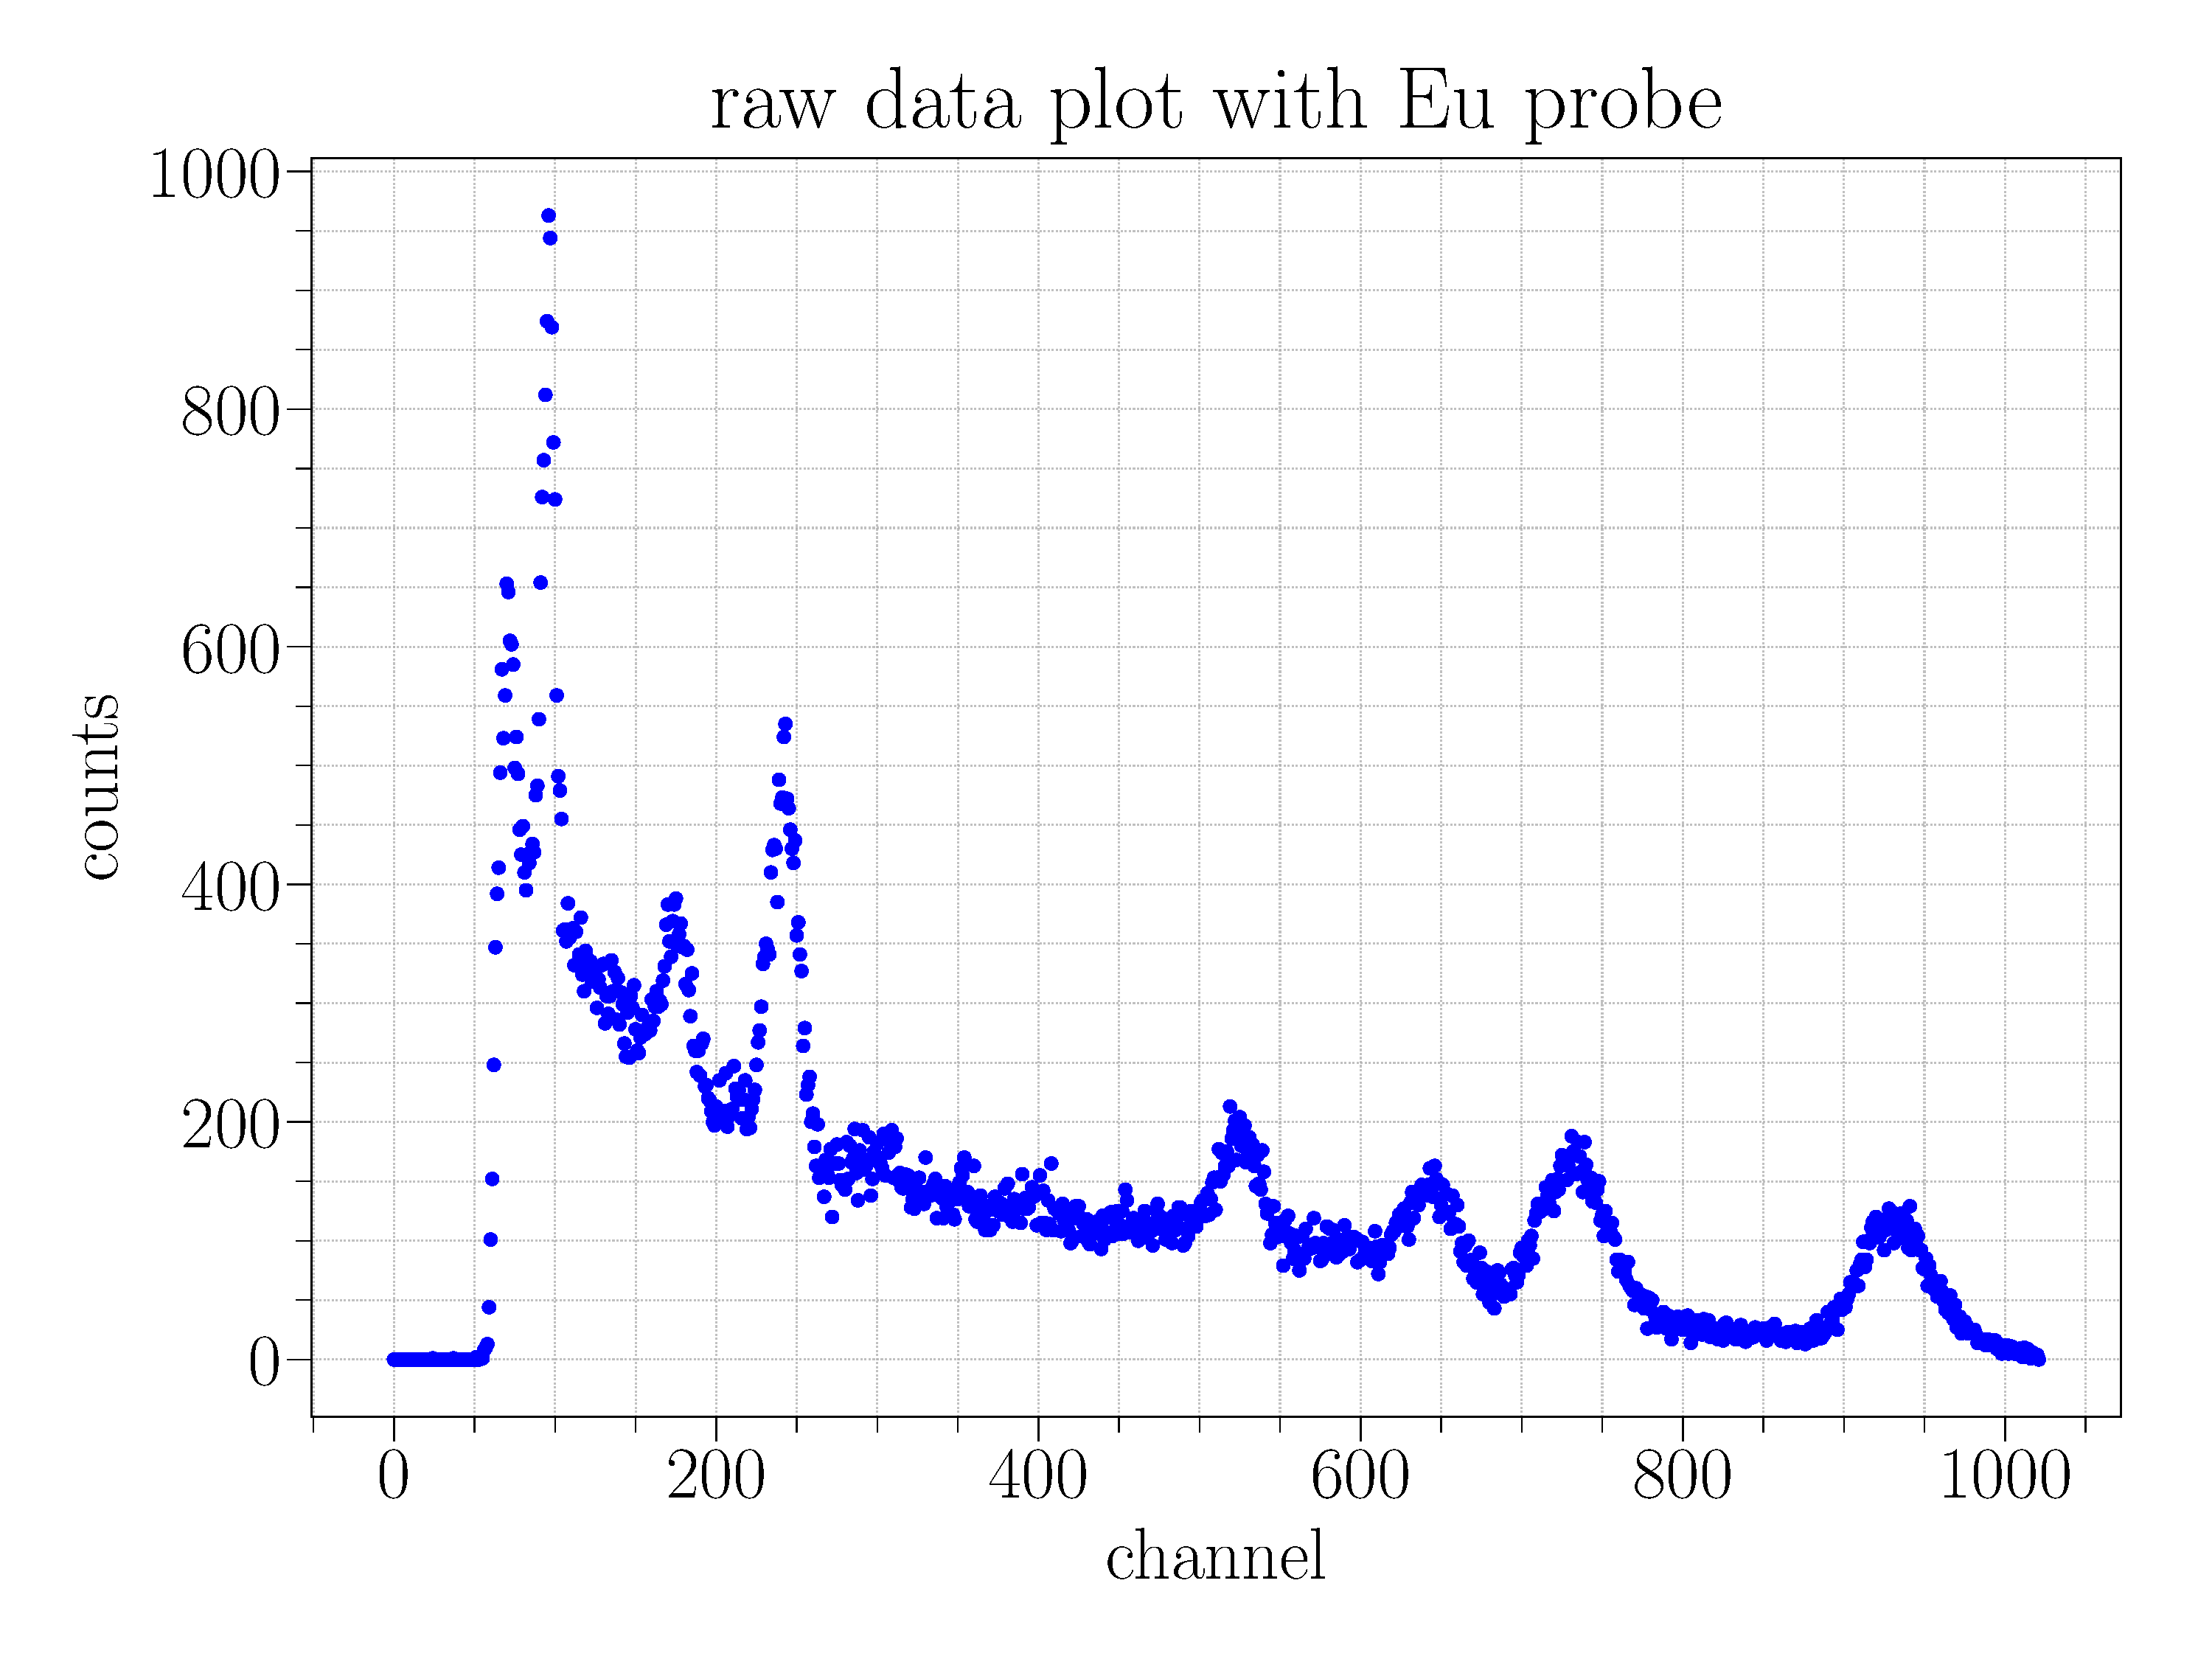
\includegraphics[scale=0.3]{../Figures/Eu_raw.pdf}
\caption{raw data with Eu probe}
\label{Eu_raw}
\end{figure}

\begin{figure}
\center
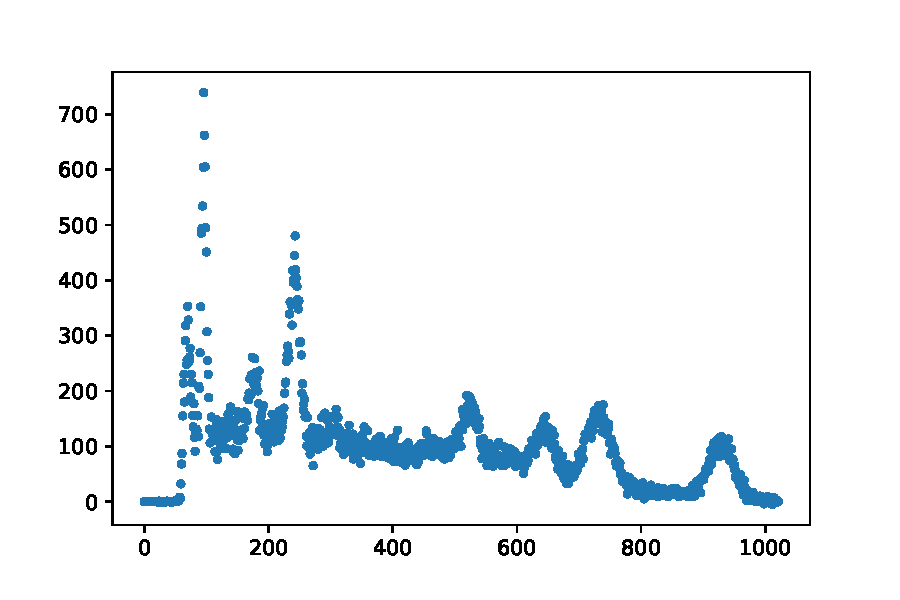
\includegraphics[scale=0.3]{../Figures/Eu.pdf}
\caption{clean data with Eu probe}
\label{Eu}
\end{figure}

\subsubsection{Calibration}
To find the channel numbers we want to use the calibration, we fit gauss distribution on the individual peaks and use the means as calibration points.
Then we proceed to do a linear fit $E_{\gamma} = a \cdot \mathrm{channel}+ b$ with $E_{\gamma}$ beeing the Energies of the peaks we identified.
The first fit, was of poor quality and based on the residuals we decided to split up the fit in two parts, which greatly improved the quality of the respective fits.

Complete fit: \newline
$a = 1.544\pm0.003$ \newline
$b = -28.334\pm1.431$ \newline
$\frac{\chi^2}{ndf} = 41.111$ \newline

Fit for lower energies: \newline
$a = 1.533\pm0.001$ \newline
$b = -25.468\pm0.322$ \newline
$\frac{\chi^2}{ndf} = 1.373$ \newline

Fit for higher energies: \newline
$a = 1.553\pm0.007$ \newline
$b = -32.815\pm5.822$ \newline
$\frac{\chi^2}{ndf} = 3.476$ \newline

\begin{figure}
\center
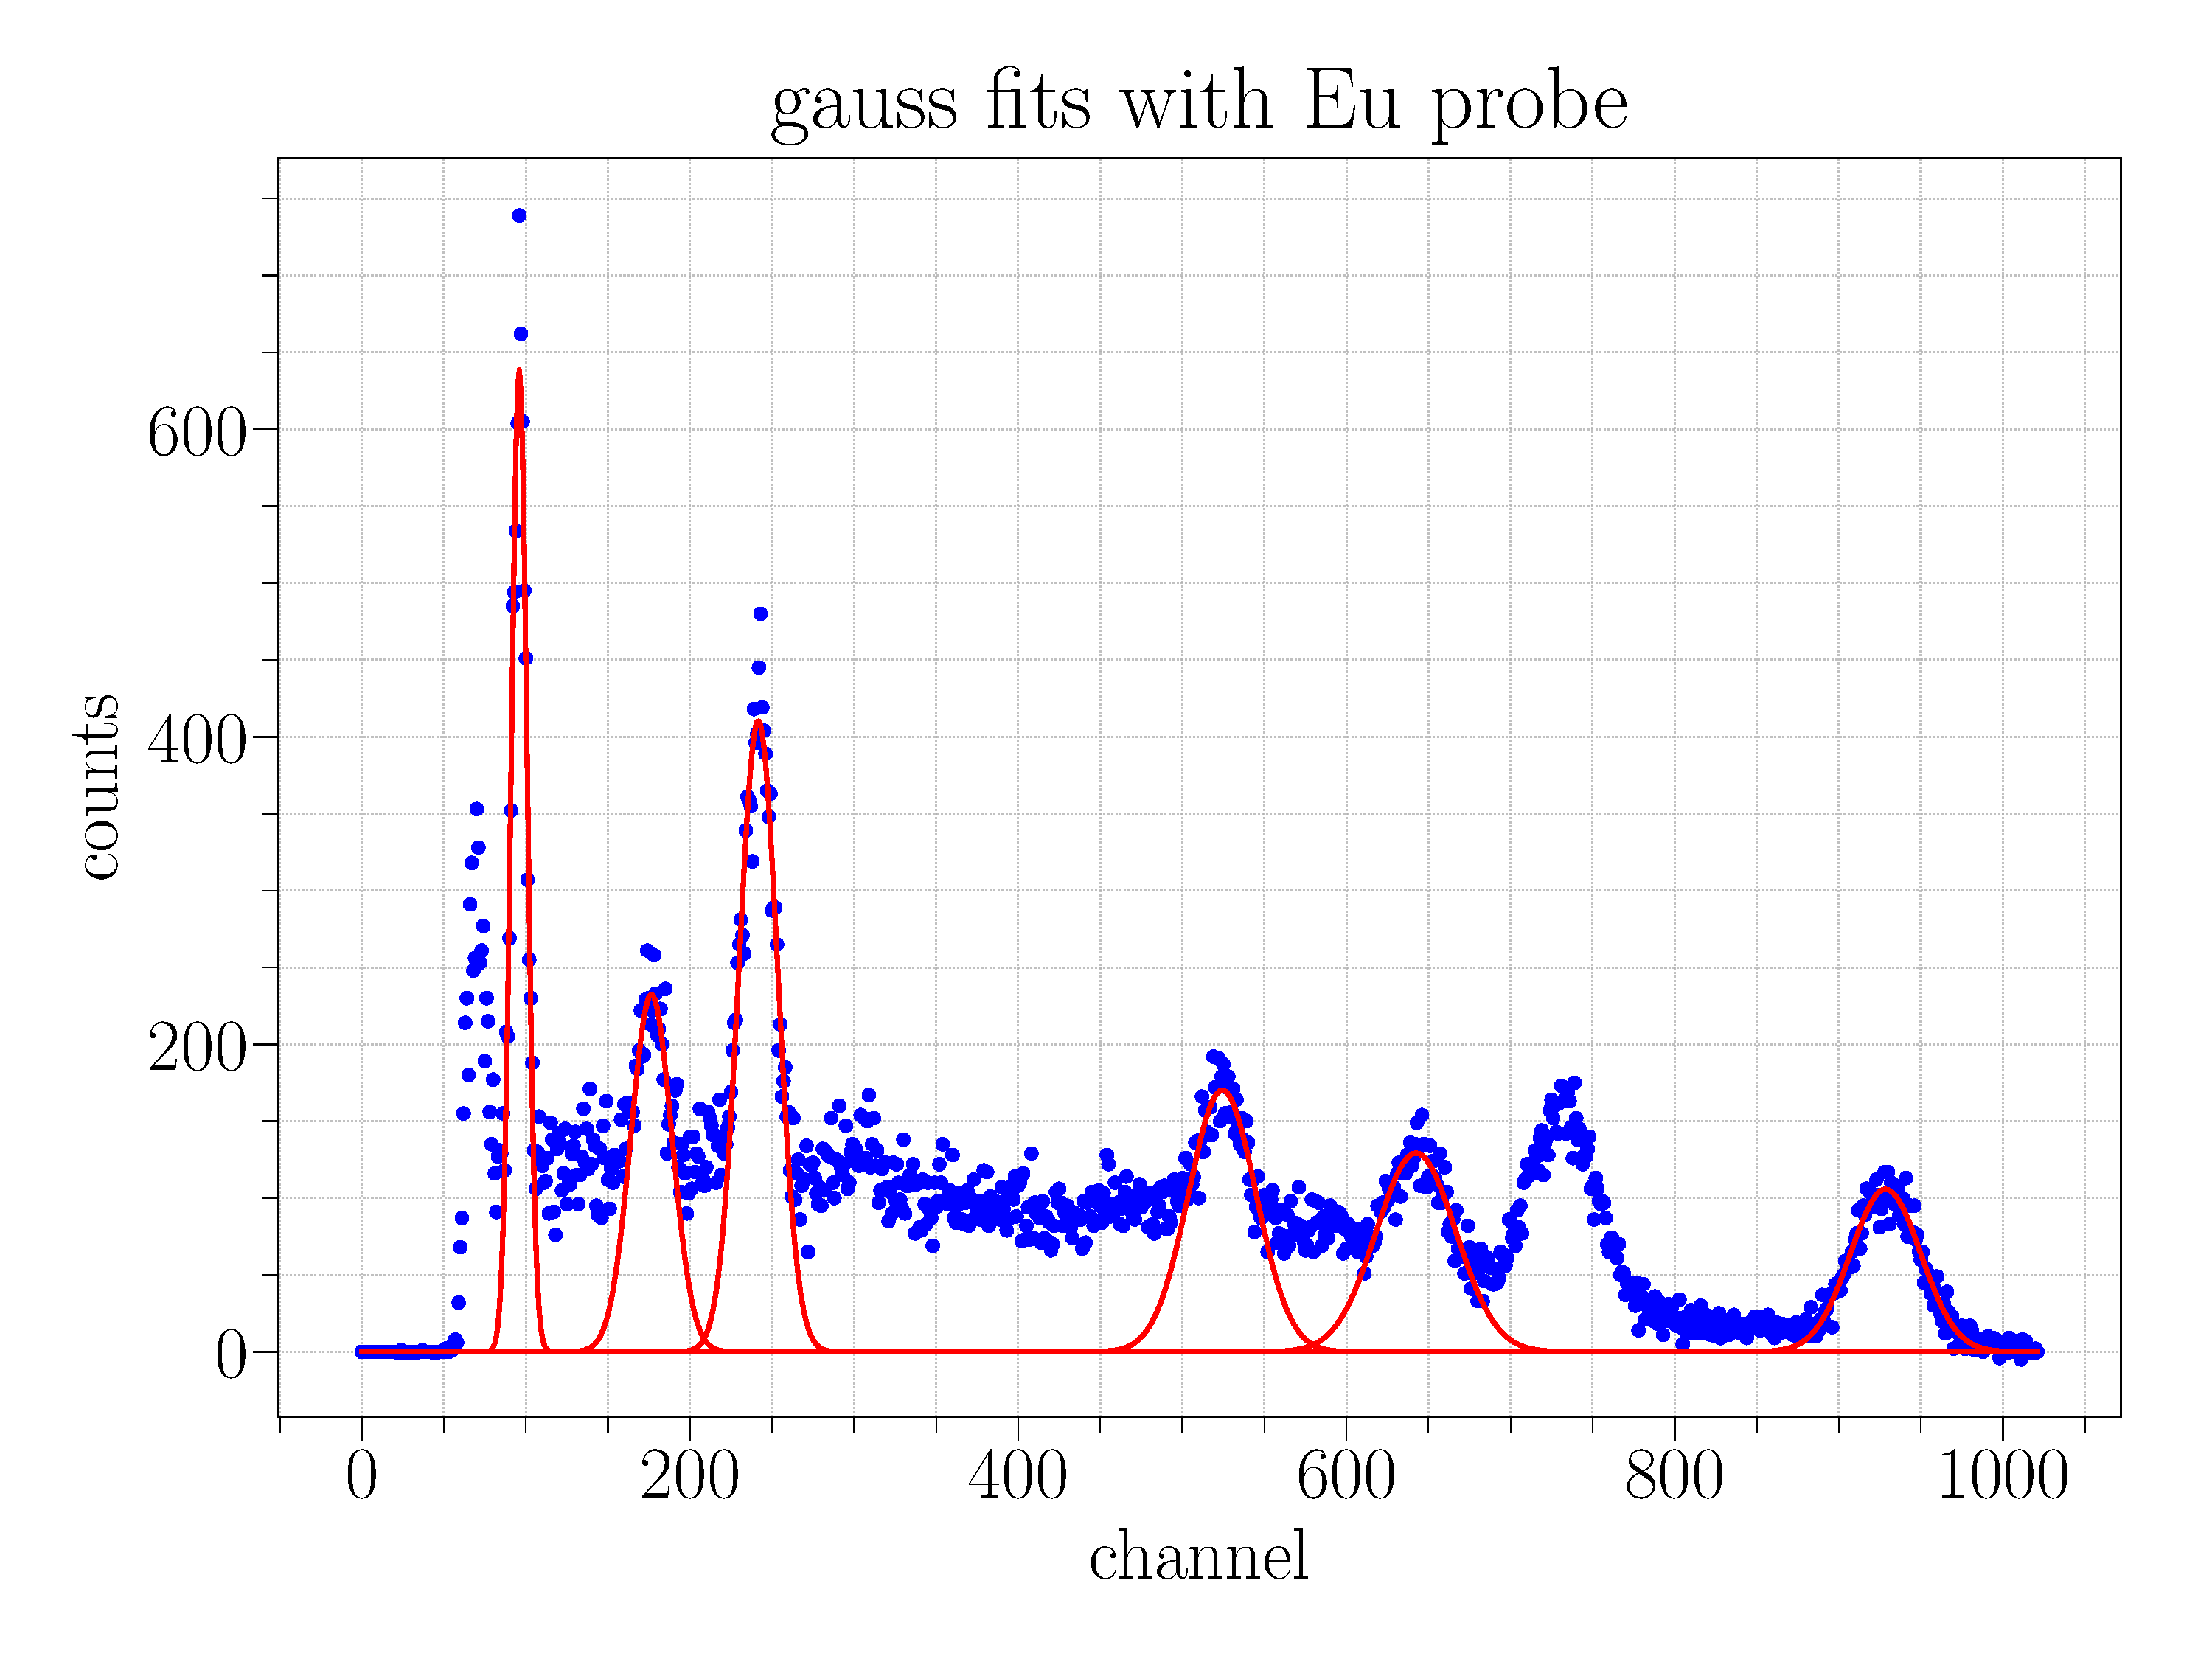
\includegraphics[scale=0.3]{../Figures/Eu_gauss.pdf}
\caption{clean data with Eu probe}
\label{Eu_gauss}
\end{figure}

\begin{figure}
\center
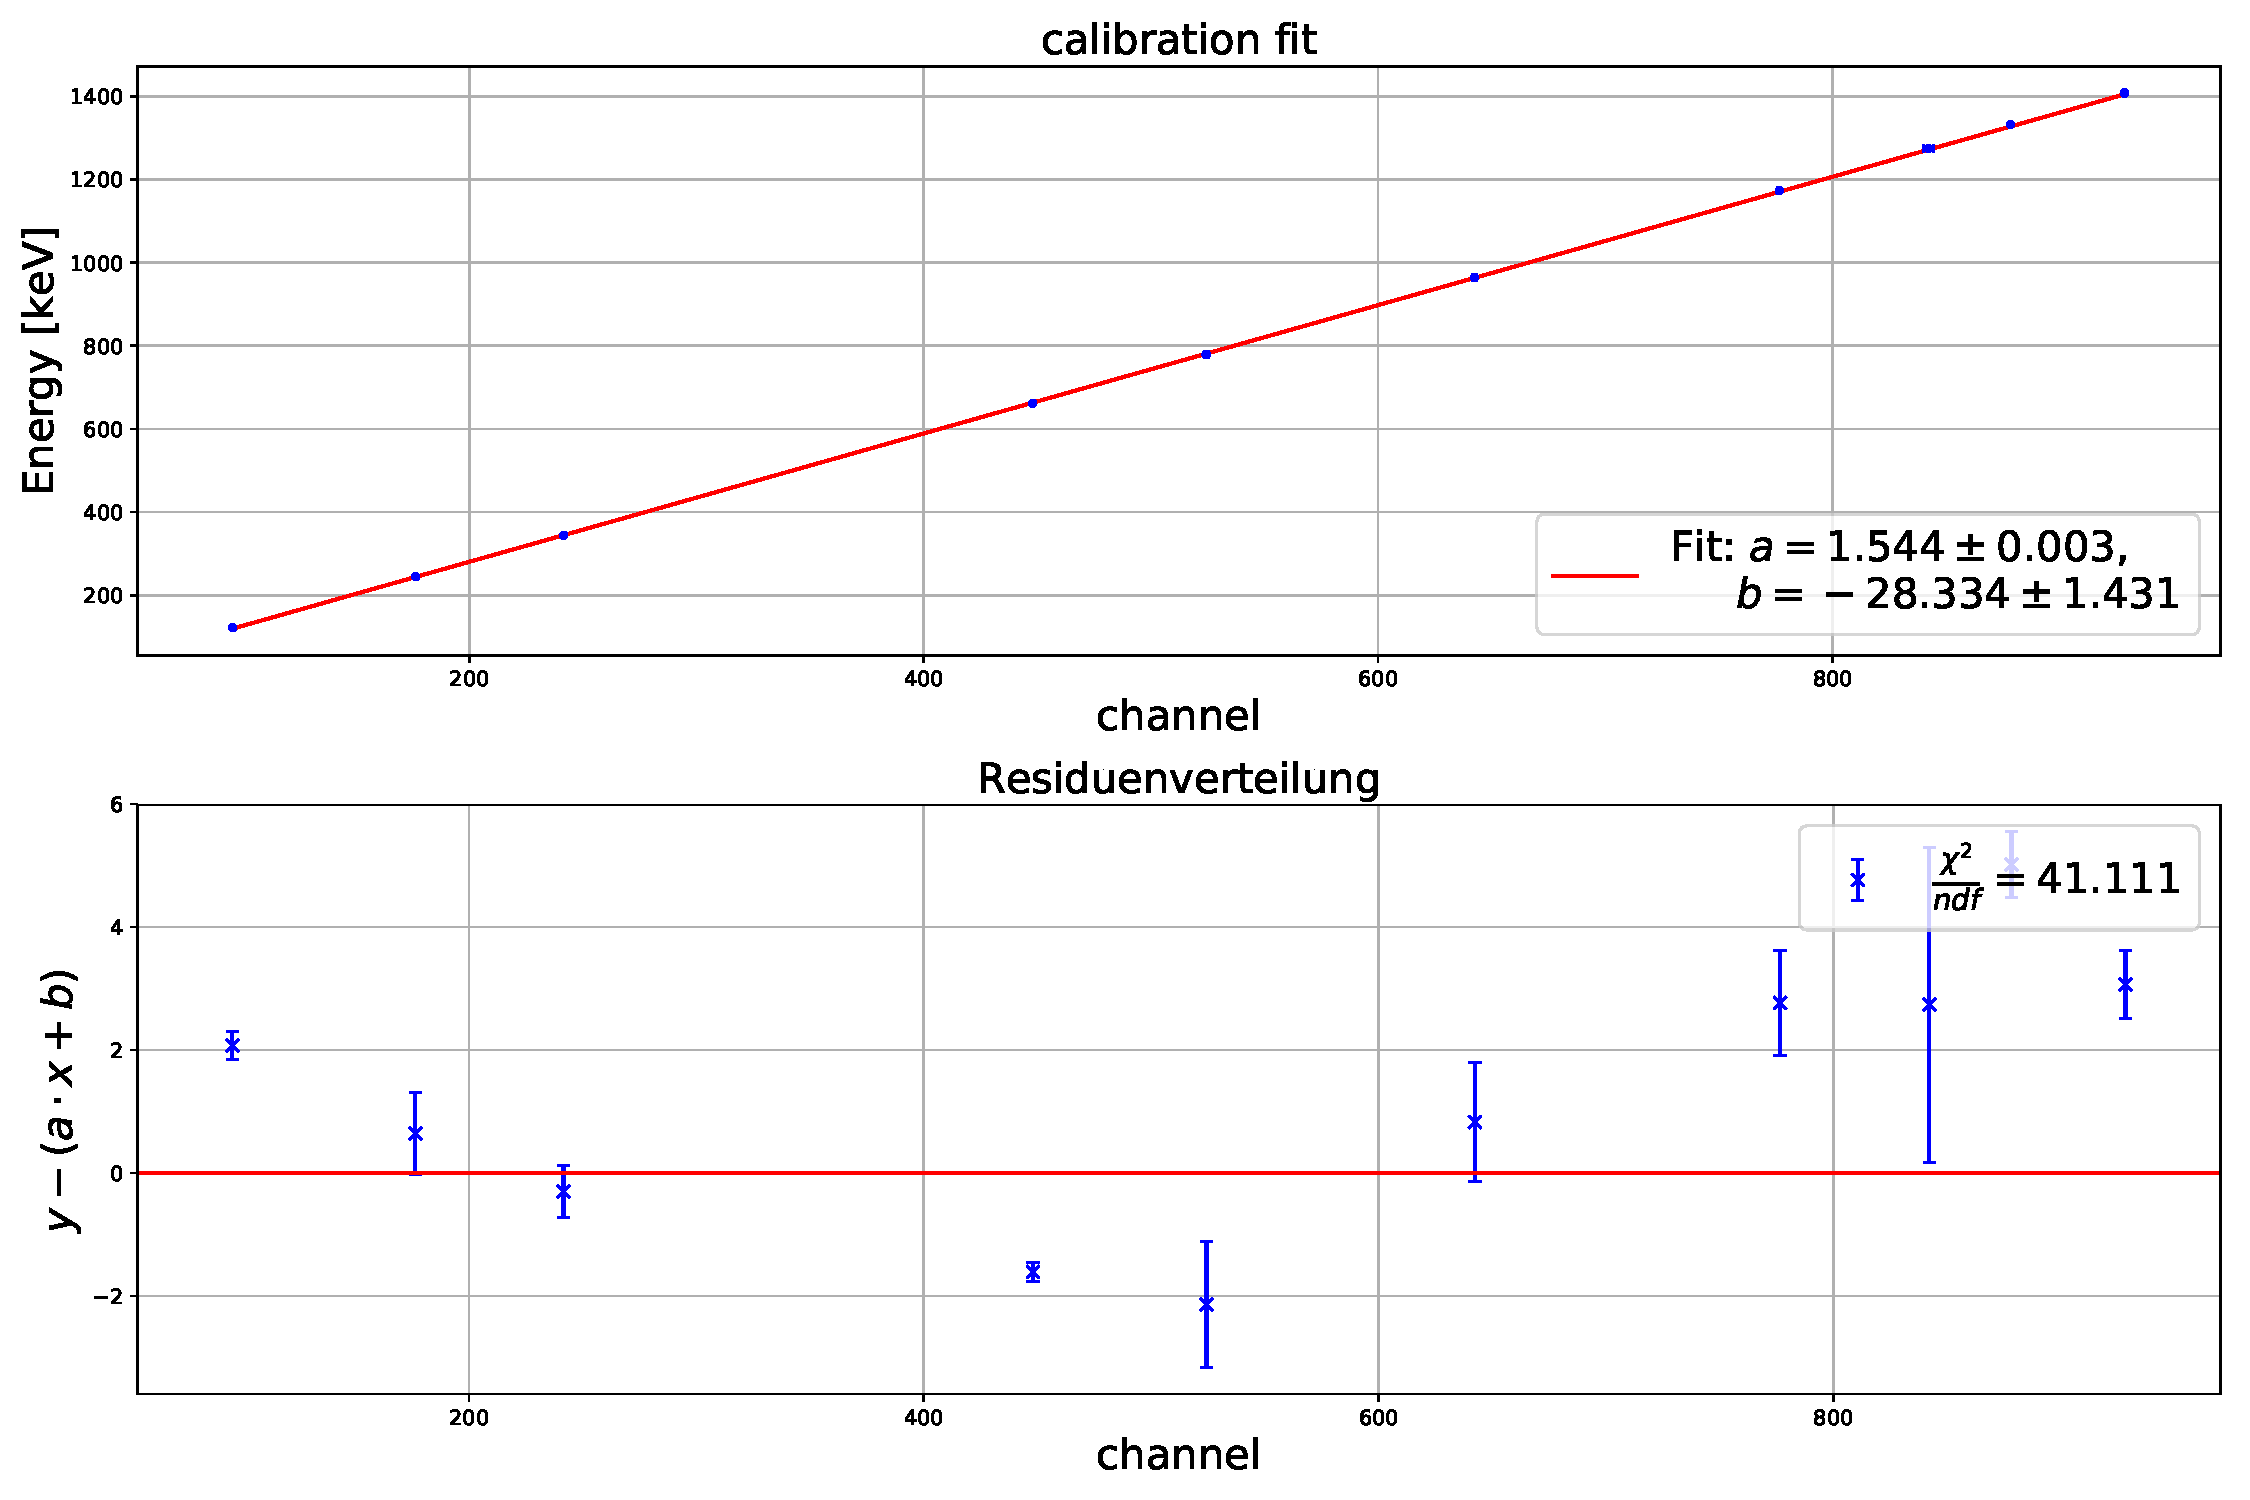
\includegraphics[scale=0.3]{../Figures/calibration fit.pdf}
\caption{linear fit for all the energies}
\label{calibFit}
\end{figure}

\begin{figure}
\center
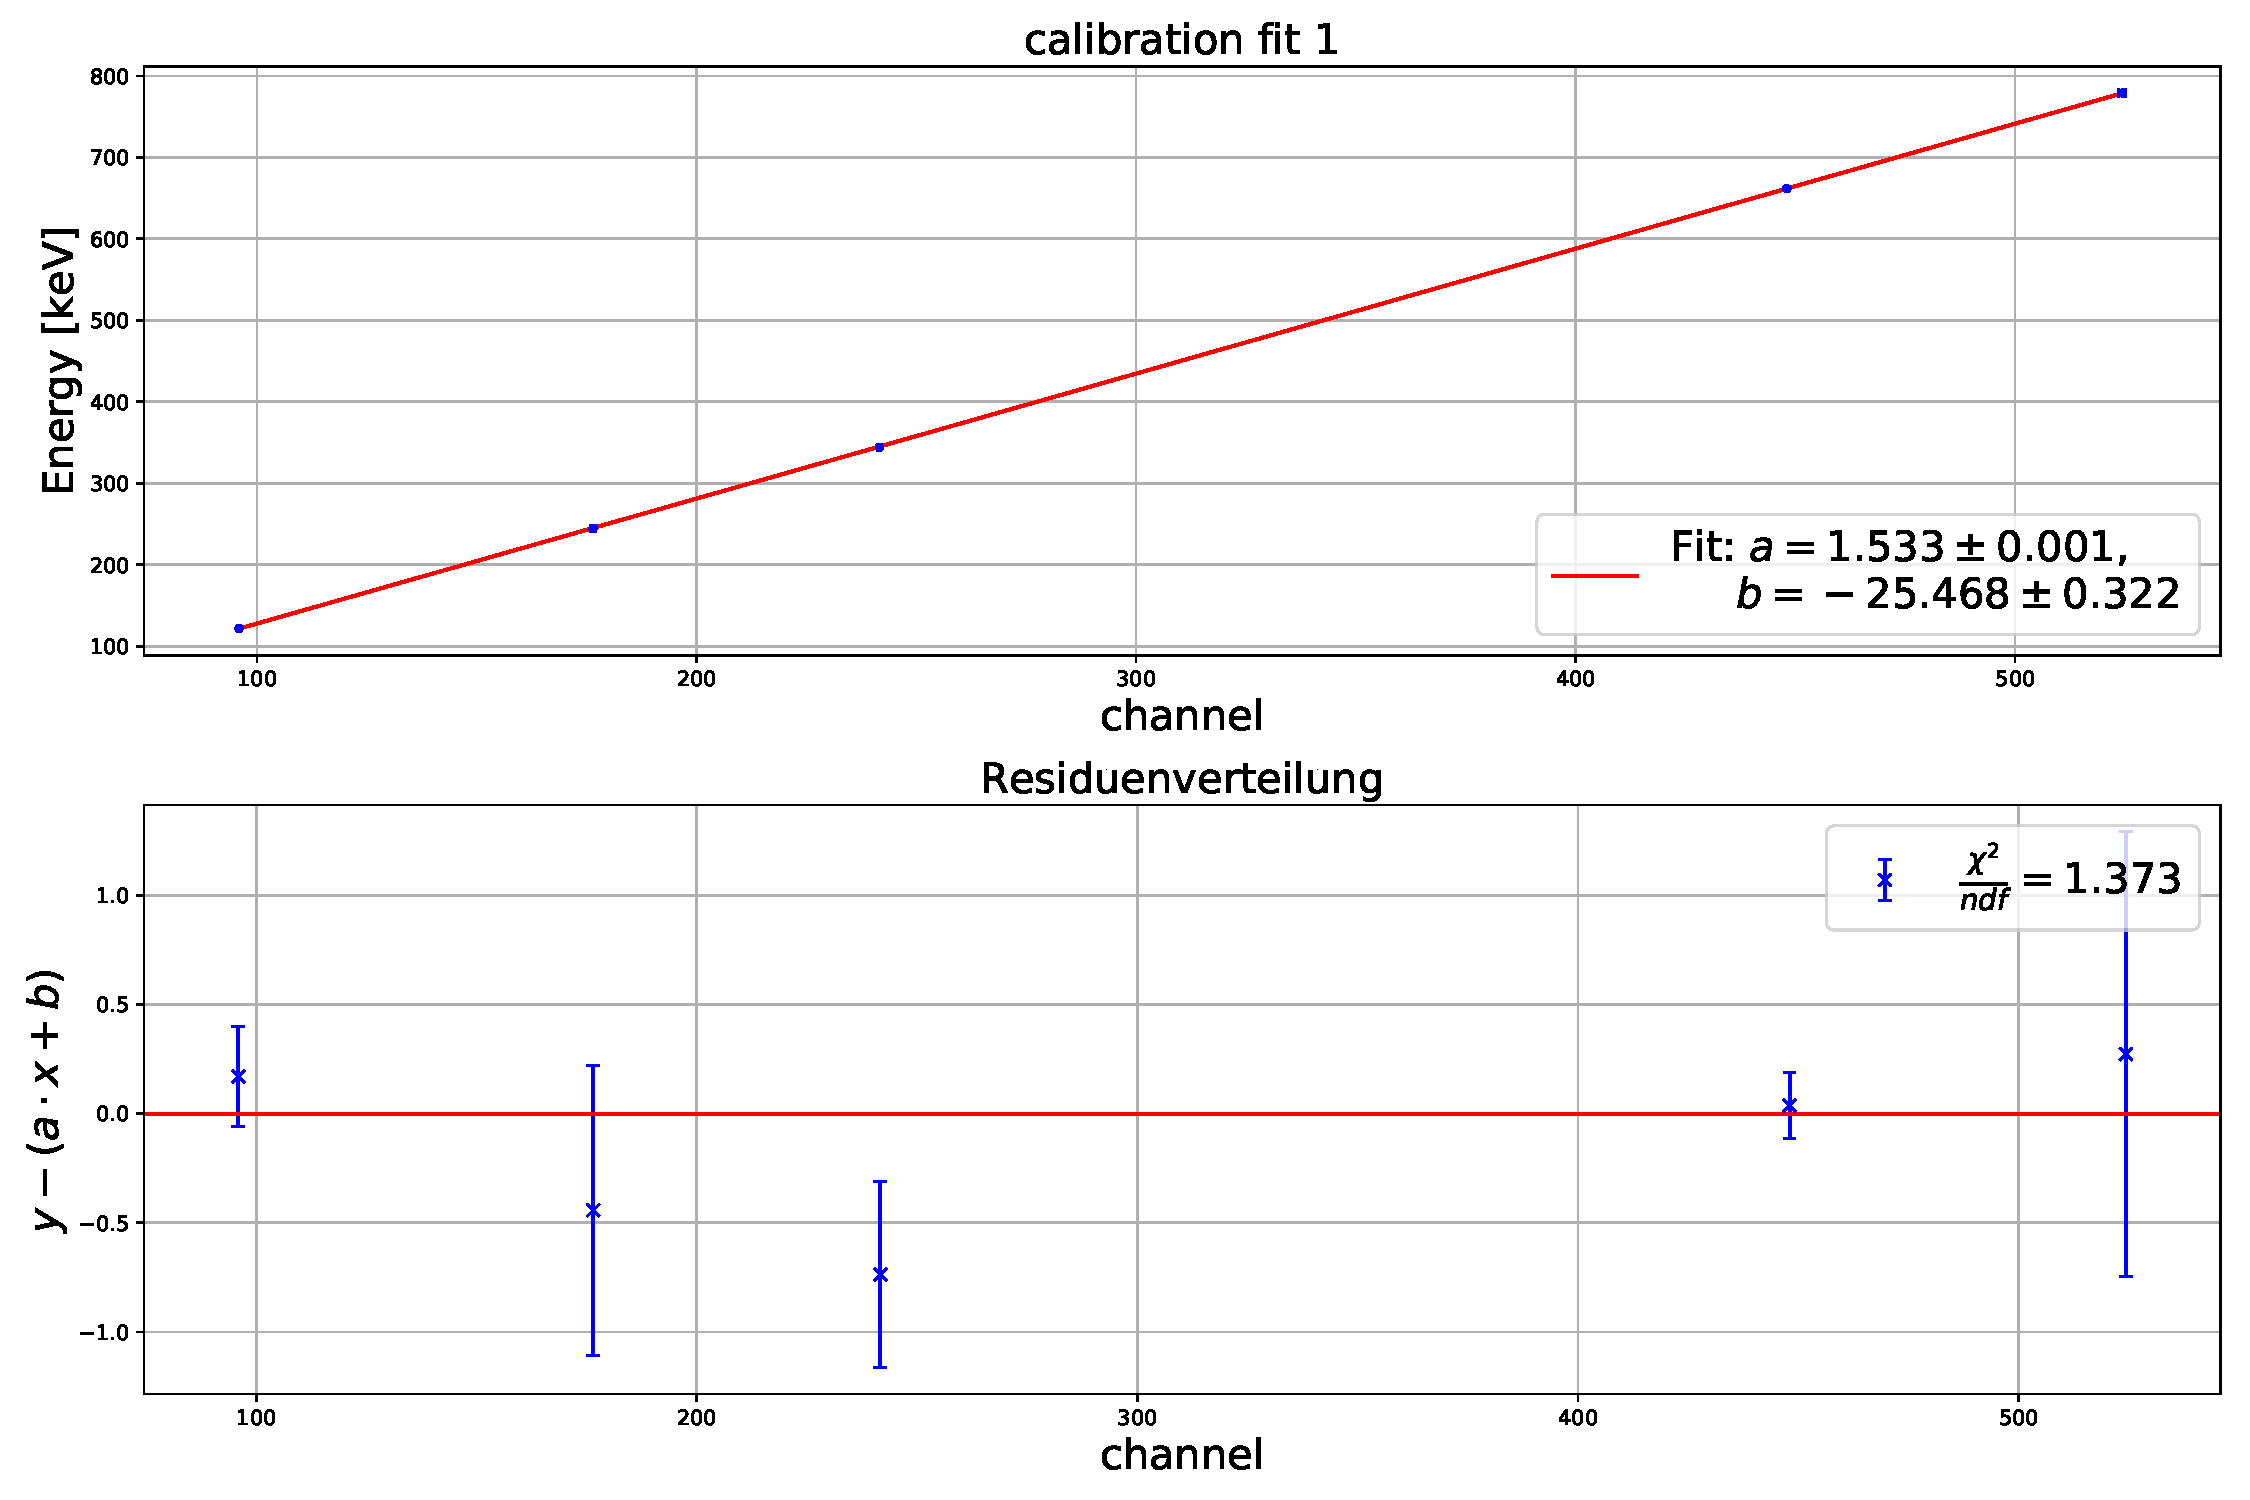
\includegraphics[scale=0.3]{../Figures/calibration fit 1.pdf}
\caption{linear fit for lower energies}
\label{calibFit}
\end{figure}

\begin{figure}
\center
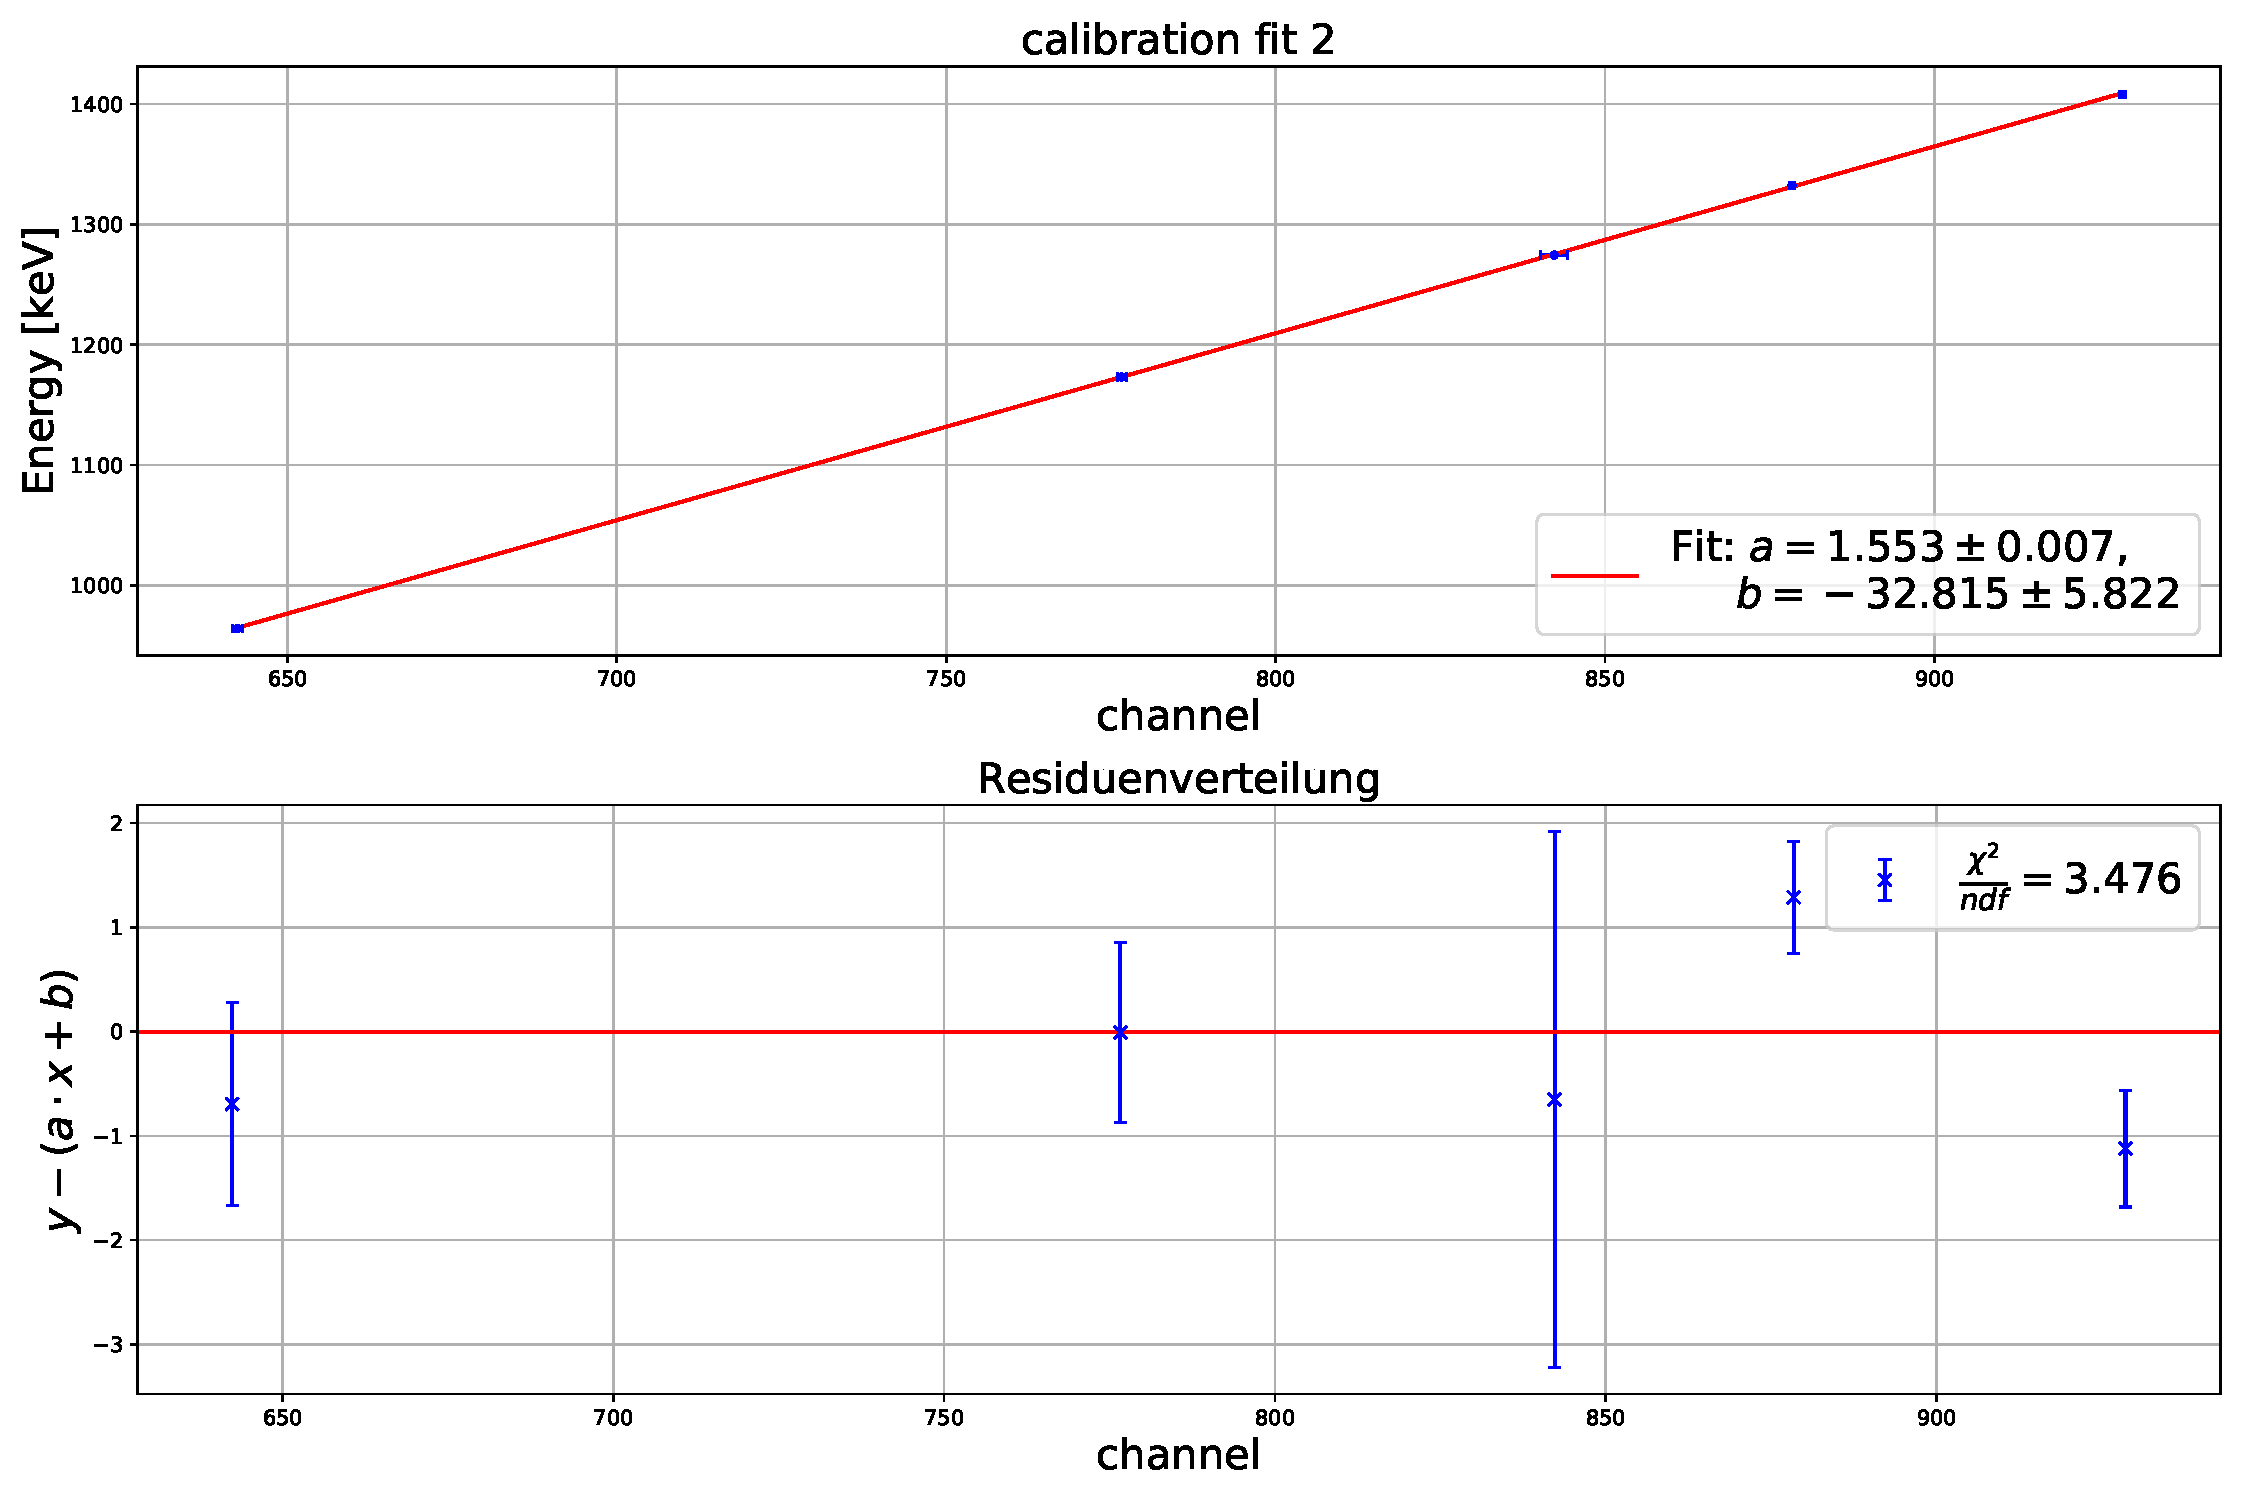
\includegraphics[scale=0.3]{../Figures/calibration fit 2.pdf}
\caption{linear fit for higher energies}
\label{calibFit}
\end{figure}

\subsubsection{Energy resolution}
We obtained the resolution by getting the standard deviations of the gauss fits and converting those to FWHM. Next we calculated the channel values at the FWHM and converted those into enrgy values based on the previous calibration. Plotting $\Delta E/E$ vs $E$ we see a decline towards higher enrgies, as it should be.
To find the constants in the resolution formula $\Delta E/E = \sqrt{a^2+b^2/E}$, we plotted $\Delta E^2$ vs $E$ and fitted the function $\Delta E^2 = a^2 \cdot E^2 + b^2 \cdot E$.
It seems the data doesn't behave quite as expected, since it doesn't fit well. Nonetheless, the values for $a$ and $b$ we get out of that fit remain our best guess for the resolution constants.\newline
fit function: \newline
$a^2 \cdot E^2 + b^2 \cdot E$ \newline
fit parameter: \newline
$a = 0.032\pm0.009$ \newline
$b = 1.766\pm0.128$ \newline
$\frac{\chi^2}{ndf} = 70.963$ \newline

\begin{figure}
\center
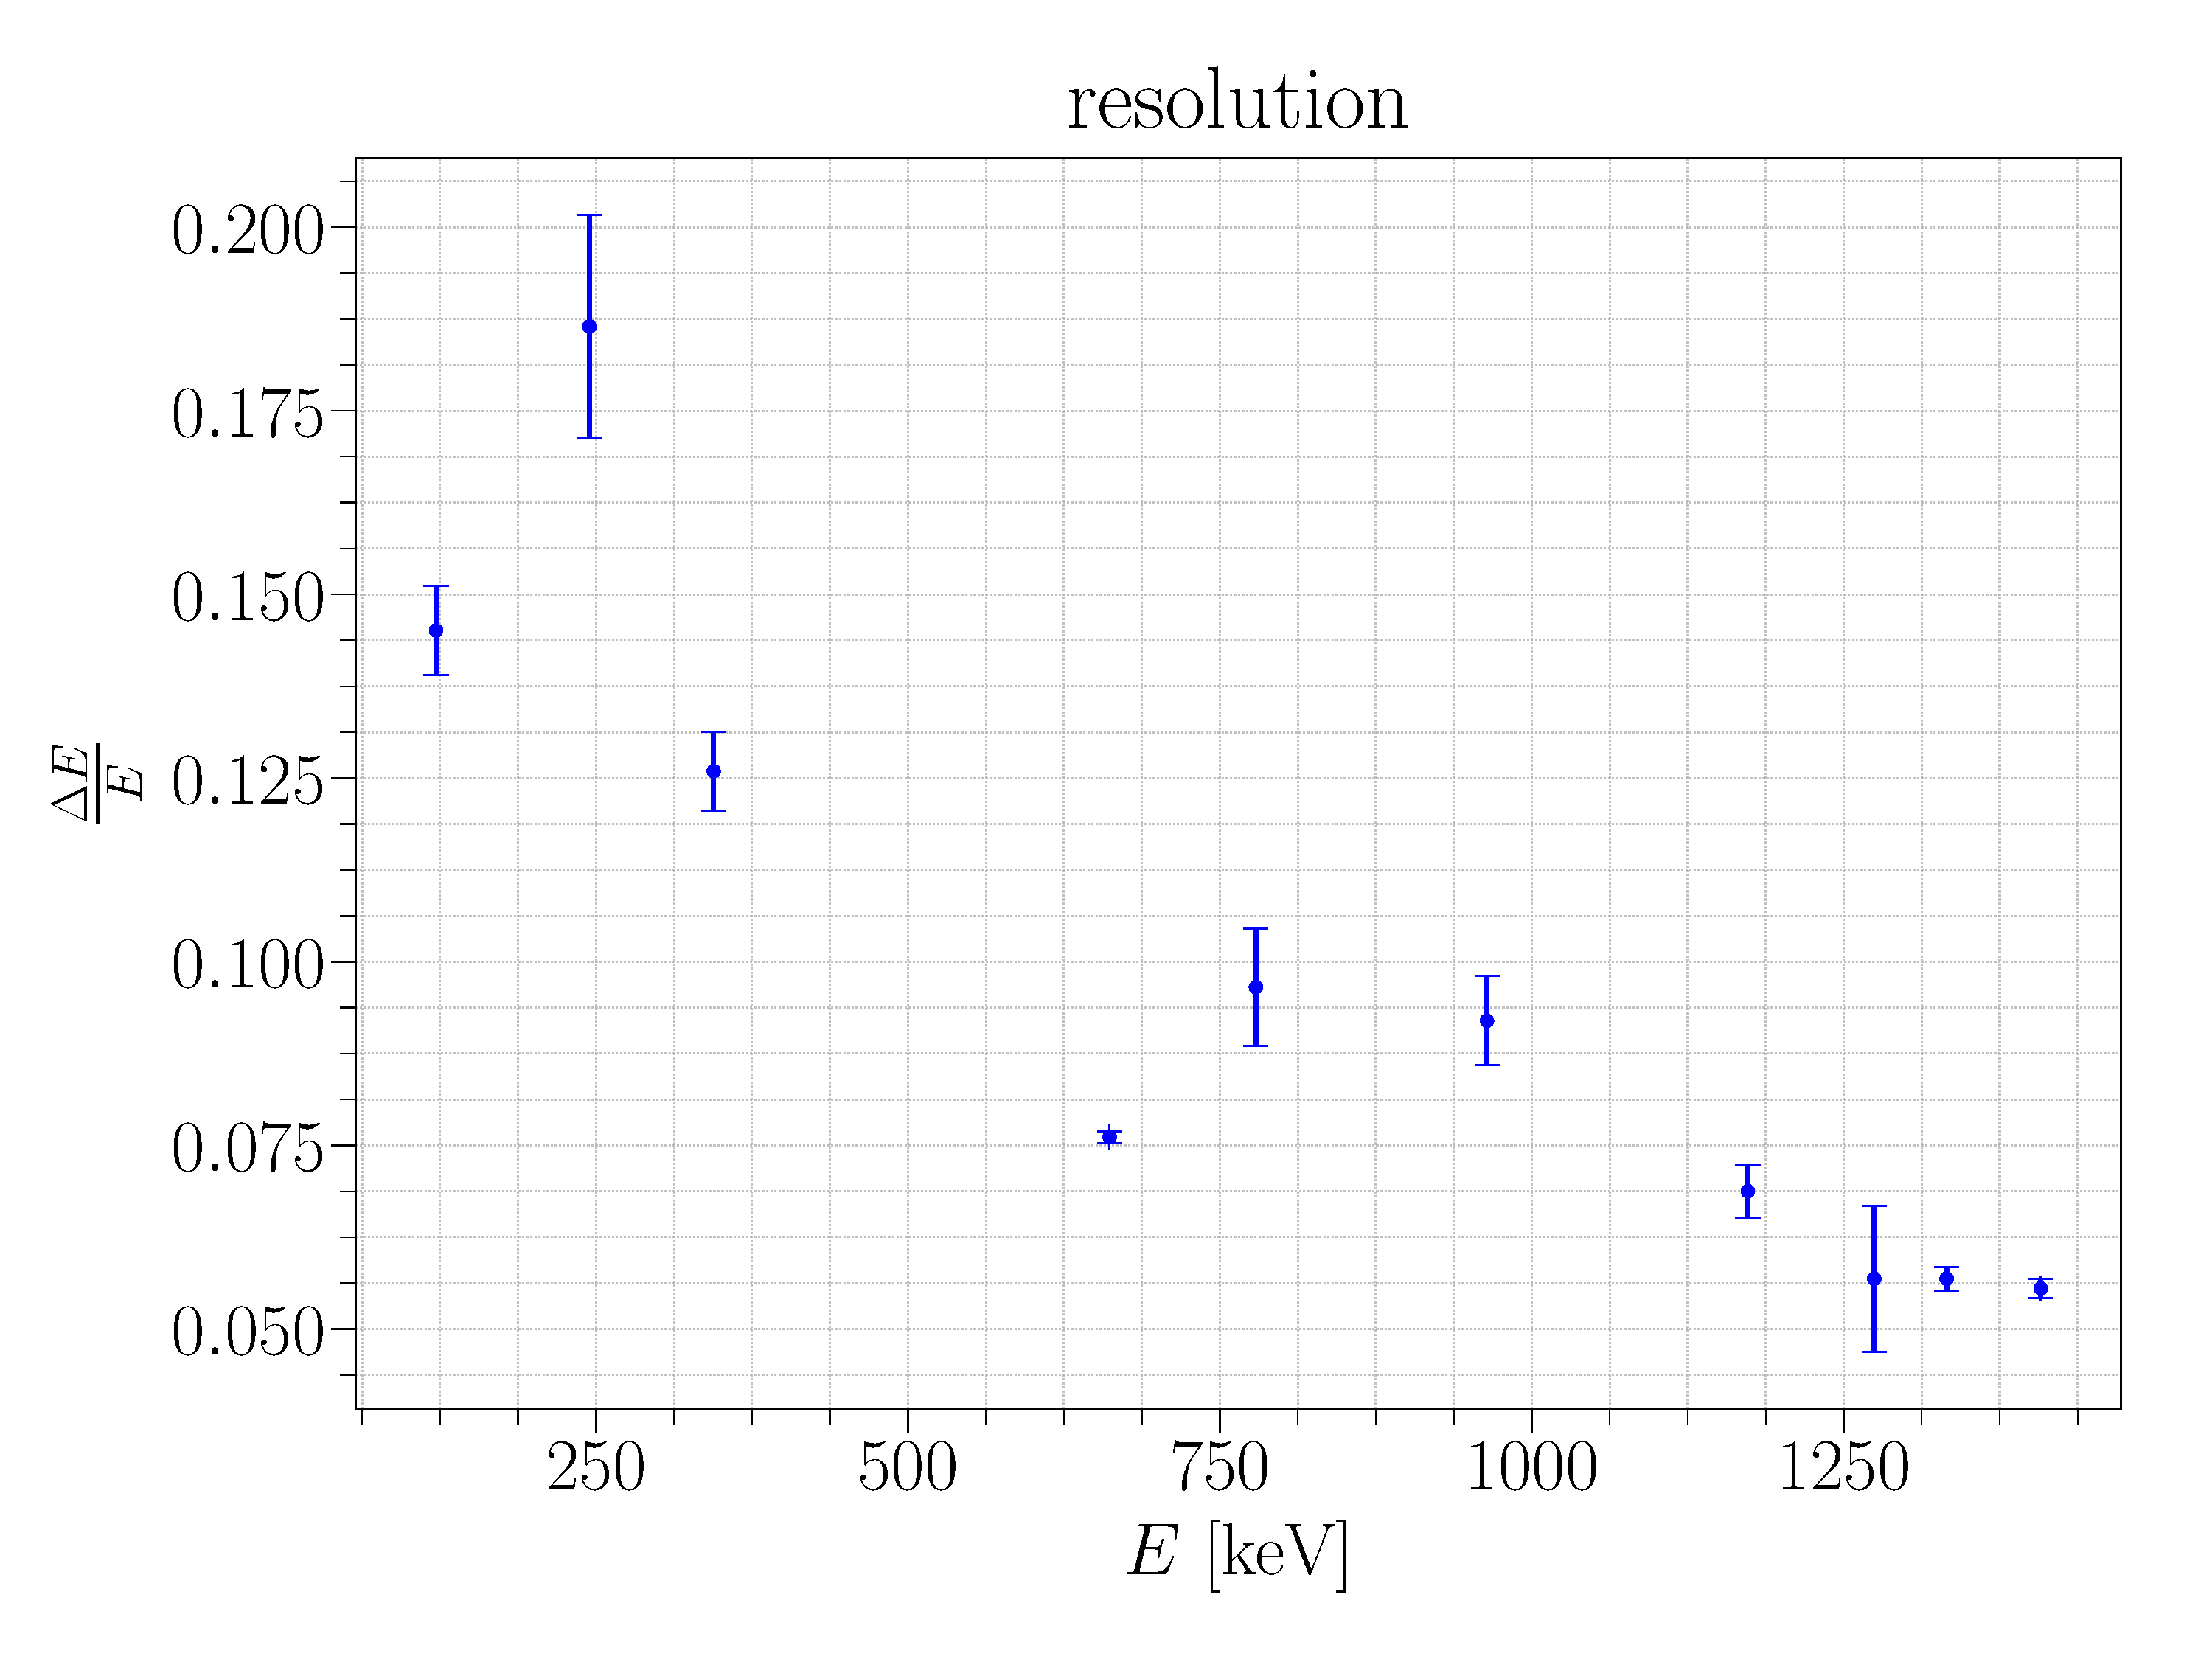
\includegraphics[scale=0.3]{../Figures/resolution.pdf}
\caption{energy resolution vs. energy}
\label{resolution}
\end{figure}
\newpage

\begin{figure}
\center
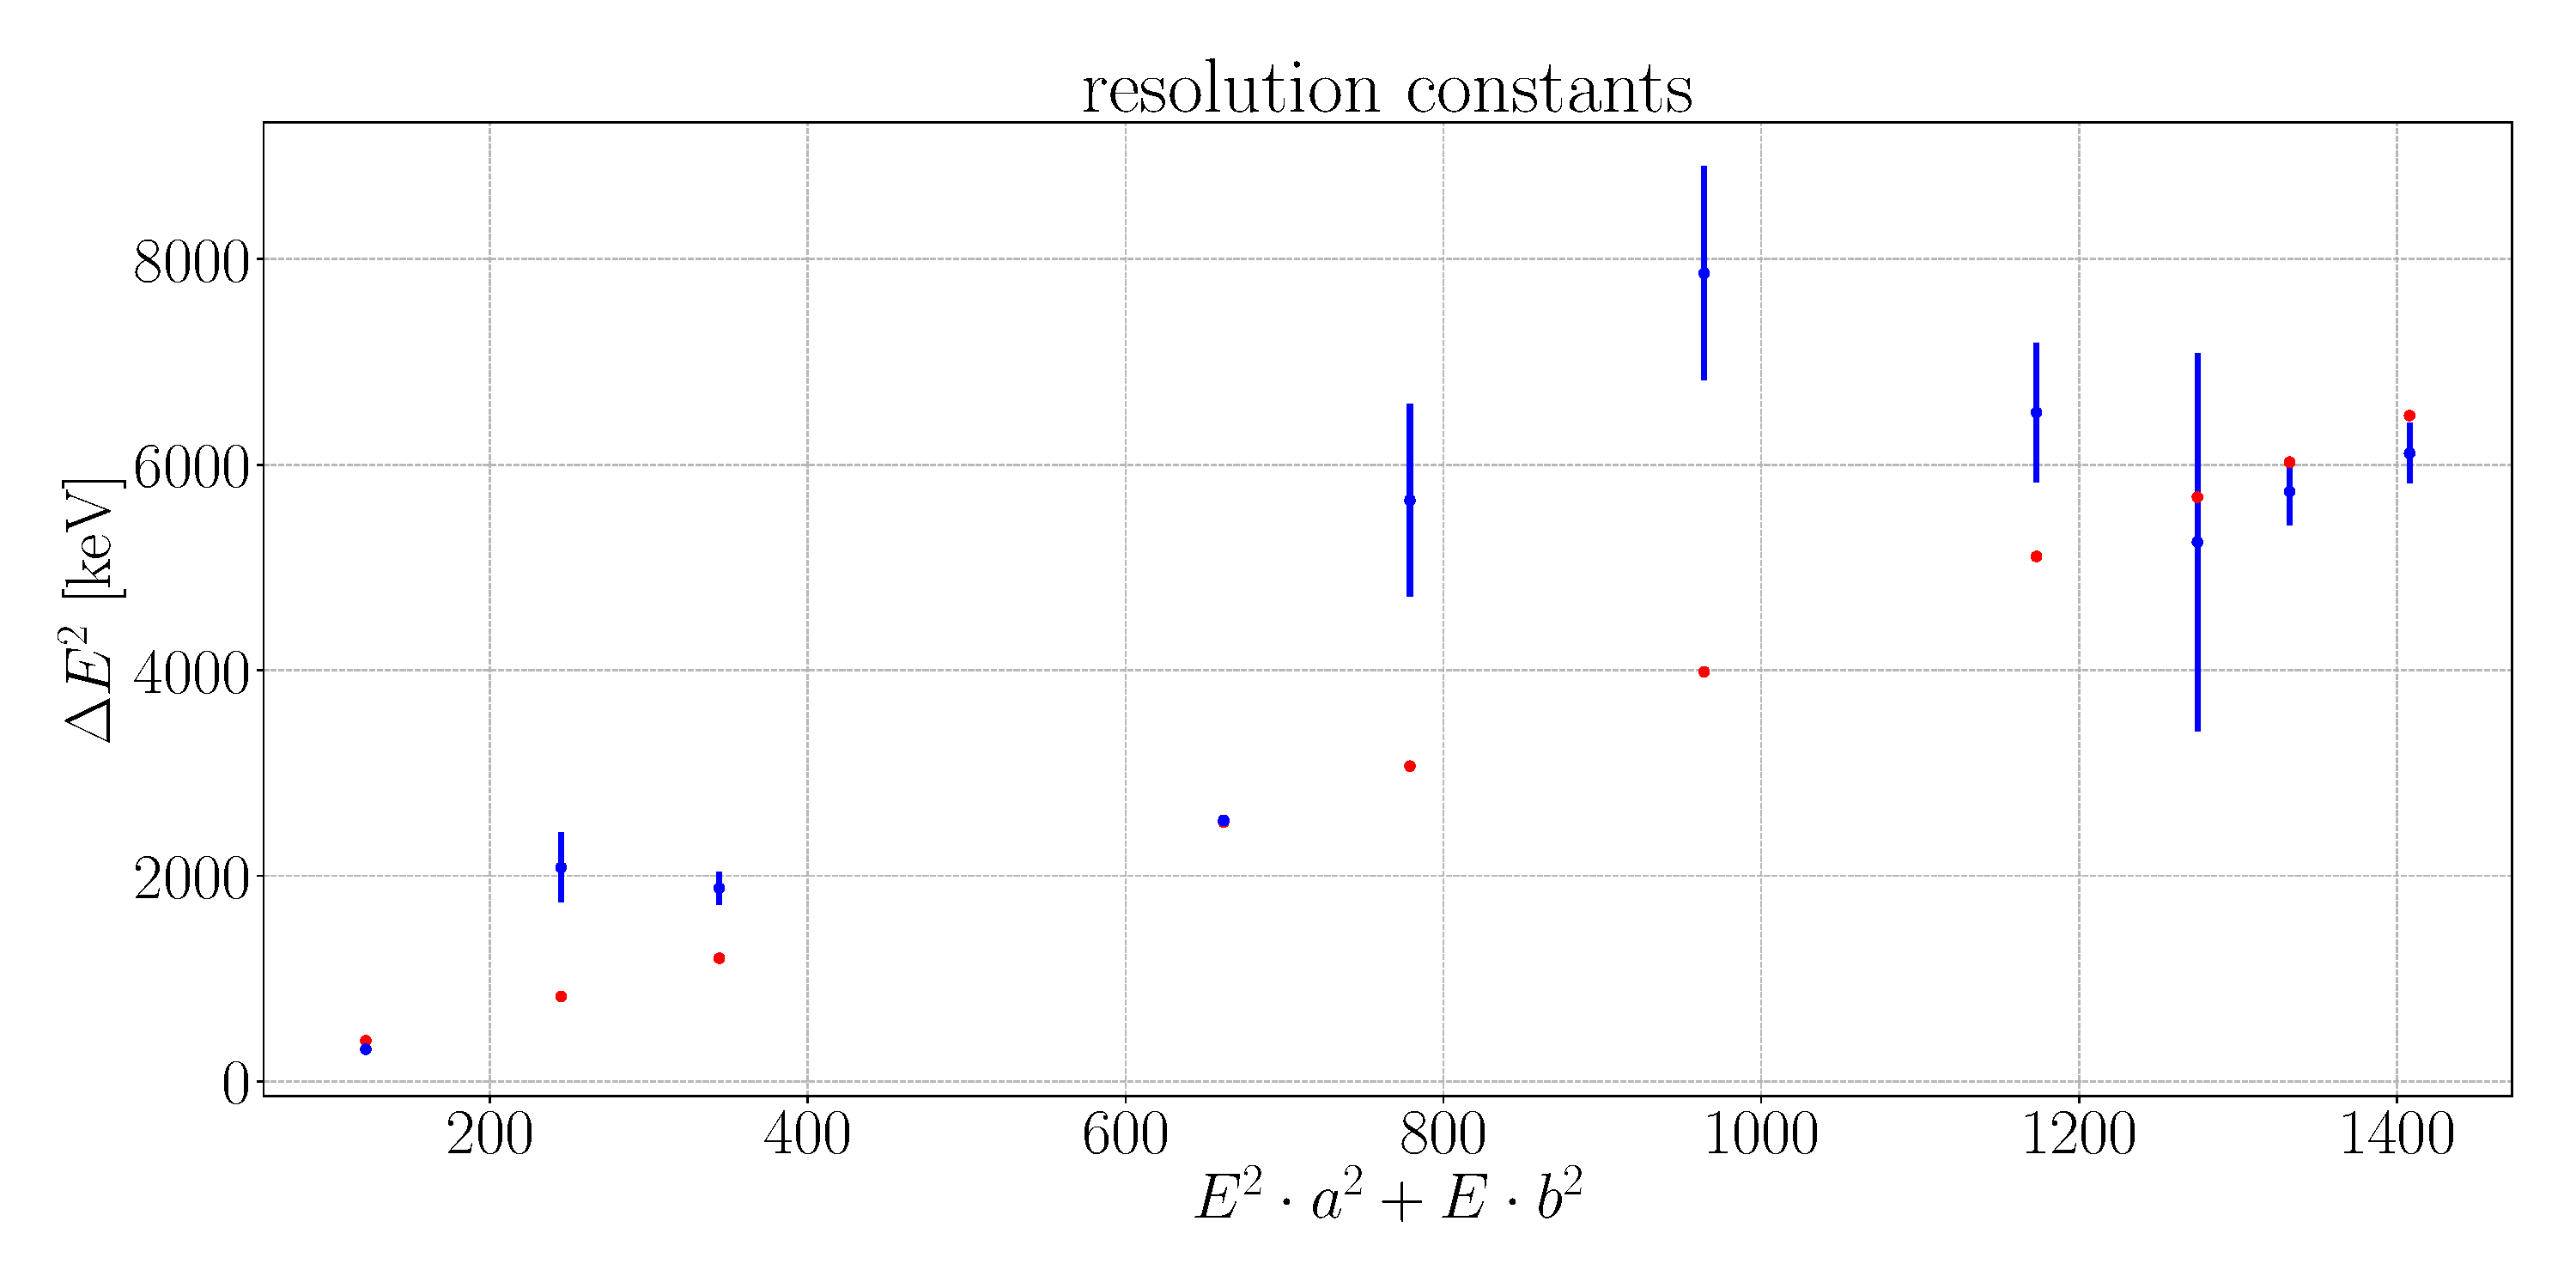
\includegraphics[scale=0.3]{../Figures/resolution constants.pdf}
\caption{linear fit to obtain constants in resolution}
\label{resolutionFit}
\end{figure}
\newpage

\subsubsection{Efficiency}

\subsubsection{Mass of the electron}
We can obtain the mass of the electron out of the anihilation peak in the sodium spectrum. It's energy is equivalent to the electron mass. 

\section{Compton scattering}

\subsection{Theory}
Energy of scattered photons: $E_\gamma^\prime = E_\gamma \cdot \frac{1}{1+a(1-\cos\theta)}$\\
count rate: $m = \frac{A \cdot I_\gamma}{4 \pi r_0^2} \cdot \eta \cdot \epsilon \cdot N_e \cdot \frac{d\sigma}{d\Omega} \cdot \frac{F_D}{r^2}$

\subsection{Setup}

\subsubsection{conventional geometry}
The source is placed on the edge of a rottary table, allowing different angles. In the middle of the table we place the scattering body (either a steel or an aluminium cylinder). To shield the radiation coming directly from the source from the detector, we use convenientl shaped lead coils.\\
Distance from source to scattering body: $r_0 = \SI{49+-1}{mm}$\\
Distance from scattering bod to detector: $r = \SI{272+-1}{mm}$\\

\subsubsection{ring geometry}
The source is aligned with the detector, but shielded of it by a lead clinder in the middle. The scattering body is an aluminium ring and the whole experiment is axially symetric.

\begin{table}[H]
	\renewcommand{\arraystretch}{1.5}
	\centering
	\begin{tabular}{|c|c|c|c|}
		\hline
		ring size & outer diameter $d_o$ & inner diameter $d_i$ & diameter $d$ \\
		\hline
		small & \SI{149+-1}{mm} & \SI{121+-1}{mm} & \SI{149+-1}{mm} \\
		\hline
		medium & \SI{199+-1}{mm} & \SI{171+-1}{mm} & \SI{149+-1}{mm} \\
		\hline
		large & \SI{250+-1}{mm} & \SI{221+-1}{mm} & \SI{149+-1}{mm} \\
		\hline
	\end{tabular}
	\caption{ }
	\label{tab:probes }
\end{table}

\subsection{Analysis}

\subsubsection{Finding scattered photons}

\begin{figure}
\center
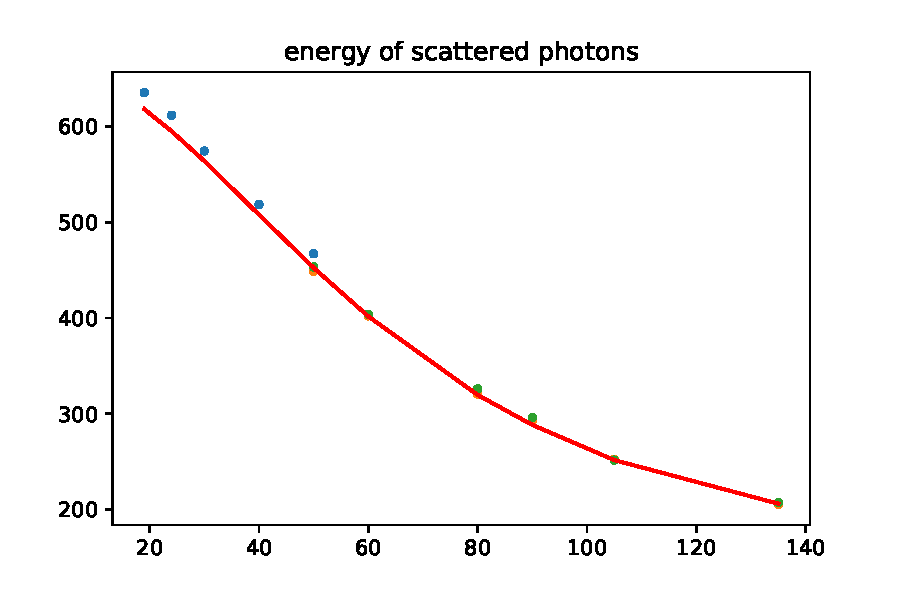
\includegraphics[scale=0.3]{../Figures/E_Phi.pdf}
\caption{Energy of scattered photons vs. scattering angle}
\label{resolution}
\end{figure}
\newpage

\subsubsection{Cross-section}

\subsubsection{Mass of the electron}

\begin{figure}
\center
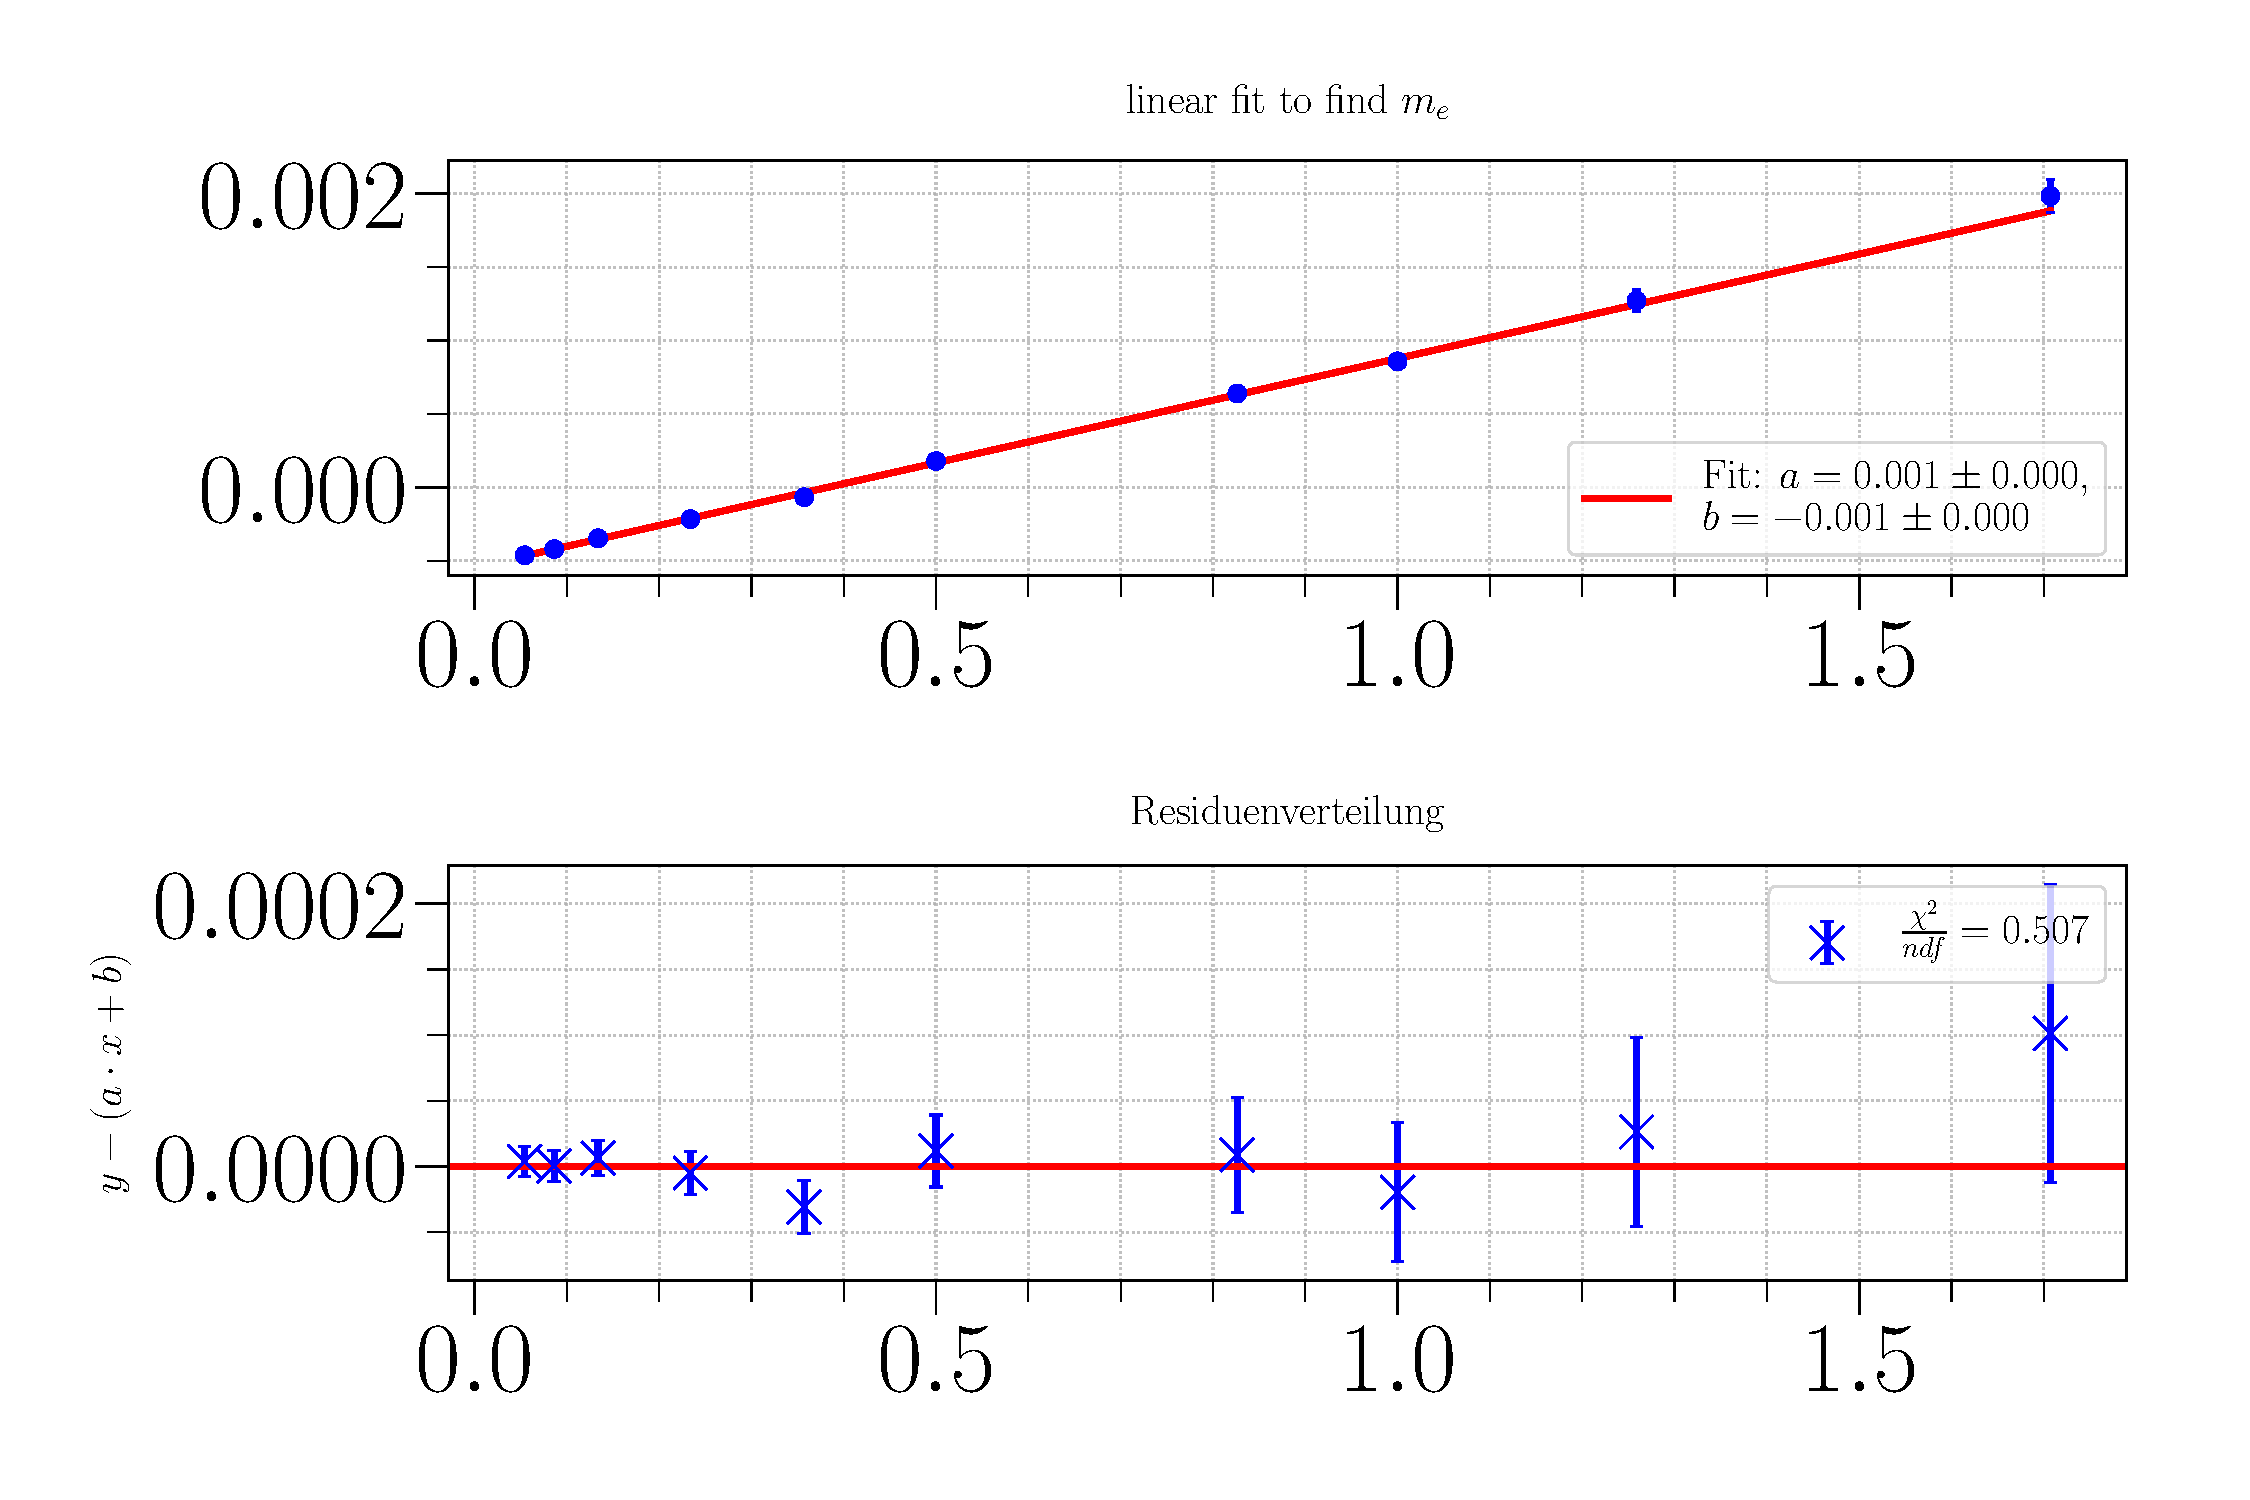
\includegraphics[scale=0.3]{../Figures/linearfittofindme.pdf}
\caption{linear fit to find the mass of the electron}
\label{meFit}
\end{figure}
\newpage






\end{document}